%!TEX root = ../main.tex

\tikzset{every picture/.style={line width=1pt}} %set default line width to 0.75pt        

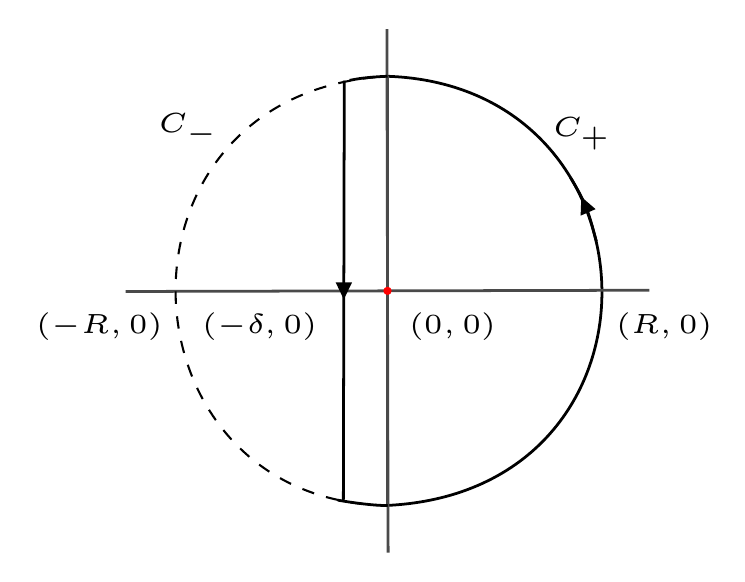
\begin{tikzpicture}[x=0.86pt,y=0.86pt,yscale=-1,xscale=1]
%uncomment if require: \path (0,357); %set diagram left start at 0, and has height of 357

%Curve Lines [id:da6356687025771366] 
\draw    (275.97,140.51) .. controls (393.49,144.53) and (398.68,314.72) .. (275.97,320.82) ;
%Straight Lines [id:da7778166164432772] 
\draw [color={rgb, 255:red, 74; green, 74; blue, 74 }  ,draw opacity=1 ]   (165.97,230.93) -- (385.97,230.41) ;
%Straight Lines [id:da7053132902182386] 
\draw [color={rgb, 255:red, 74; green, 74; blue, 74 }  ,draw opacity=1 ]   (276.23,340.67) -- (275.71,120.67) ;
%Straight Lines [id:da3860117988849814] 
\draw [color={rgb, 255:red, 74; green, 74; blue, 74 }  ,draw opacity=1 ]   (275.97,140.51) -- (275.97,320.82) ;
%Curve Lines [id:da8696519251258394] 
\draw [line width=0.75]  [dash pattern={on 4.5pt off 4.5pt}]  (275.97,320.82) .. controls (161.04,319.39) and (153.49,147.13) .. (275.97,140.51) ;
%Straight Lines [id:da885594660241974] 
\draw    (257.81,142.33) -- (257.42,318.61) ;
\draw [shift={(257.61,234.27)}, rotate = 270.13] [fill={rgb, 255:red, 0; green, 0; blue, 0 }  ][line width=0.08]  [draw opacity=0] (7.14,-3.43) -- (0,0) -- (7.14,3.43) -- cycle    ;
%Curve Lines [id:da01957205219237279] 
\draw    (260.05,142.23) .. controls (265.49,141.06) and (271.33,140.68) .. (275.97,140.51) ;
%Curve Lines [id:da7685319347743758] 
\draw    (275.97,320.82) .. controls (271.82,321.03) and (262.09,319.86) .. (255.08,318.61) ;
%Curve Lines [id:da9382254876031242] 
\draw    (352.85,183.1) .. controls (360.63,195.56) and (361.15,201.09) .. (363.74,209.91) ;
\draw [shift={(357.4,191.16)}, rotate = 66.46] [fill={rgb, 255:red, 0; green, 0; blue, 0 }  ][line width=0.08]  [draw opacity=0] (7.14,-3.43) -- (0,0) -- (7.14,3.43) -- cycle    ;
%Shape: Ellipse [id:dp016643737096258437] 
\draw  [color={rgb, 255:red, 255; green, 0; blue, 0 }  ,draw opacity=1 ][fill={rgb, 255:red, 255; green, 0; blue, 0 }  ,fill opacity=1 ] (274.86,230.67) .. controls (274.86,230.05) and (275.36,229.56) .. (275.97,229.56) .. controls (276.58,229.56) and (277.08,230.05) .. (277.08,230.67) .. controls (277.08,231.28) and (276.58,231.78) .. (275.97,231.78) .. controls (275.36,231.78) and (274.86,231.28) .. (274.86,230.67) -- cycle ;

% Text Node
\draw (125.36,236.93) node [anchor=north west][inner sep=0.75pt]  [font=\normalsize,xscale=2,yscale=2]  {\fontsize{4.5}{4}\selectfont$(-R,0)$};
% Text Node
\draw (282.08,236.93) node [anchor=north west][inner sep=0.75pt]  [font=\tiny,xscale=2,yscale=2] [align=left] {\fontsize{4.5}{4}\selectfont$( 0,0)$};
% Text Node
\draw (195.08,236.93) node [anchor=north west][inner sep=0.75pt]  [font=\tiny,xscale=2,yscale=2] [align=left] {\fontsize{4.5}{4}\selectfont$(-\delta,0)$};
% Text Node
\draw (369,236.93) node [anchor=north west][inner sep=0.75pt]  [font=\tiny,xscale=2,yscale=2]  {\fontsize{4.5}{4}\selectfont$(R,0)$};
% Text Node
\draw (342.5,154.9) node [anchor=north west][inner sep=0.75pt]  [font=\tiny,xscale=2,yscale=2]  {$\mathscr{C}_{+}$};
% Text Node
\draw (176.83,153.4) node [anchor=north west][inner sep=0.75pt]  [font=\tiny,xscale=2,yscale=2]  {$C_{-}$};

\end{tikzpicture}